\documentclass[a4paper,11pt]{article}
\usepackage{fancyhdr}
\usepackage{fancyheadings}
\usepackage[american]{babel}
\usepackage[utf8]{inputenc}
\usepackage[active]{srcltx}
\usepackage{algorithm}
\usepackage[noend]{algorithmic}
\usepackage{amsmath}
\usepackage{amssymb}
\usepackage{amsthm}
\usepackage{bbm}
\usepackage{enumerate}
\usepackage{graphicx}
\usepackage{ifthen}
\usepackage{listings}
\usepackage{struktex}
\usepackage{hyperref}

\usepackage{braket}

\renewcommand{\vector}[2]{{\left(\begin{array}{c} #1 \\ #2 \end{array}\right)}}

%%%%%%%%%%%%%%%%%%%%%%%%%%%%%%%%%%%%%%%%%%%%%%%%%%%%%%
%%%%%%%%%%%%%% EDIT THIS PART %%%%%%%%%%%%%%%%%%%%%%%%
%%%%%%%%%%%%%%%%%%%%%%%%%%%%%%%%%%%%%%%%%%%%%%%%%%%%%%
\newcommand{\Fach}{Basics of Quantum Information and Computing}
\newcommand{\Name}{Michael Hartmann}
\newcommand{\Lehrstuhl}{Theoretische Physik I, Universität Augsburg}
\newcommand{\Uebungsblatt}{7} %  <-- UPDATE ME
\newcommand{\Date}{21.12.2016} %  <-- UPDATE ME
%%%%%%%%%%%%%%%%%%%%%%%%%%%%%%%%%%%%%%%%%%%%%%%%%%%%%%
%%%%%%%%%%%%%%%%%%%%%%%%%%%%%%%%%%%%%%%%%%%%%%%%%%%%%%

\DeclareMathOperator{\Tr}{Tr}

\setlength{\parindent}{0em}
\setlength{\parskip}{1em}
\topmargin -1.0cm
\oddsidemargin 0cm
\evensidemargin 0cm
\setlength{\textheight}{9.2in}
\setlength{\textwidth}{6.0in}

%%%%%%%%%%%%%%%
%% Problem-COMMAND
\newcommand{\Problem}[1]{
  {
  \vspace*{0.5cm}
  \textsf{\textbf{Problem #1}}
  \vspace*{0.2cm}
  
  }
}
%%%%%%%%%%%%%%
\hypersetup{
    pdftitle={\Fach{}: Exercise \Uebungsblatt{}},
    pdfauthor={\Name},
    pdfborder={0 0 0}
}

\lstset{ %
language=java,
basicstyle=\footnotesize\tt,
showtabs=false,
tabsize=2,
captionpos=b,
breaklines=true,
extendedchars=true,
showstringspaces=false,
flexiblecolumns=true,
}

\title{Exercise \Uebungsblatt{}}
\author{\Name{}}

\begin{document}
\thispagestyle{fancy}
\lhead{\sf \Fach{} \\ \tiny{\Name, \Lehrstuhl}}
\rhead{\sf \Date{}}
\vspace*{0.2cm}
\begin{center}
\LARGE \sf \textbf{Exercise \Uebungsblatt{} -- Interaction-free Measurement}
\end{center}
\vspace*{0.2cm}

%%%%%%%%%%%%%%%%%%%%%%%%%%%%%%%%%%%%%%%%%%%%%%%%%%%%%%
%% Insert your solutions here %%%%%%%%%%%%%%%%%%%%%%%%
%%%%%%%%%%%%%%%%%%%%%%%%%%%%%%%%%%%%%%%%%%%%%%%%%%%%%%

We usually think of a measurement as an interaction between an object and a
measuring device. However, there is also another way to measure -- without
interaction.
\begin{figure}[h!]
\centering

\includegraphics[scale=0.44]{images/slit2.png}
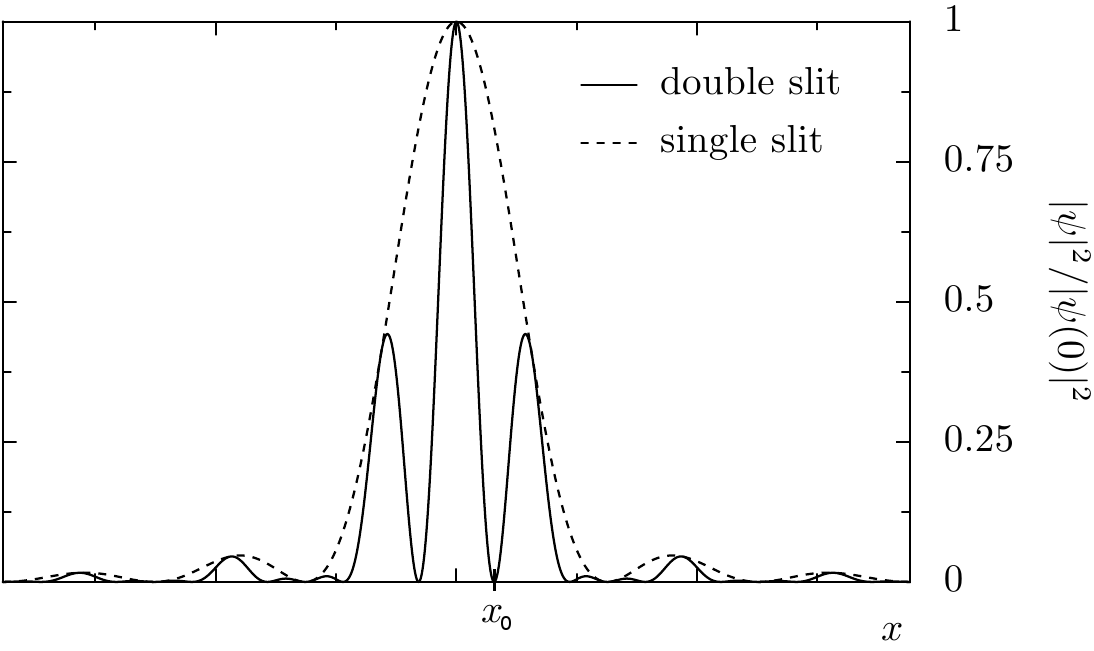
\includegraphics[scale=0.24]{images/slit.png}
\caption{left: a cat is blocking a slit in a double-slit experiment, right: probability of measuring a photon dependent on position for the single and double-slit experiment}
\end{figure}
Consider a double-slit experiment as seen in Fig. 1. Let $x_0$ be one minimum
of the interference pattern. If we place a detector at $x=x_0$, and let the
source emit photon by photon, then no photon will reach the detector. Now,
consider a cat blocking one of the slits. There is no more interference, hence,
there is a possibility for a photon to reach the detector. If a photon reaches
the detector, the photon has not interacted with the object, yet we know, that
the cat is blocking the slit. We've seen the cat {\it in the dark}.

In the following we will consider interaction-free measurements with
Mach-Zehnder interferometers.
\begin{enumerate}[a)]
\item The Mach-Zehnder interferometer in Fig. 2 consists of two beam splitters
(B1 and B2) and two mirrors (M). The path lengths in the upper and lower arms of
the interferometer are the same.

\begin{figure}[h!]
\centering
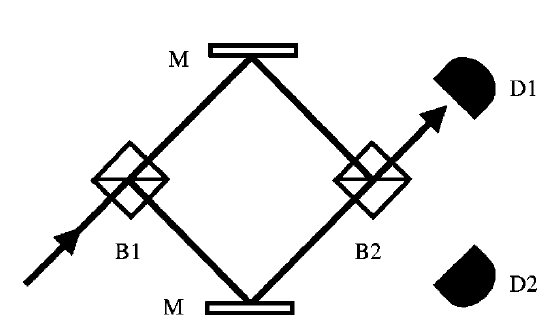
\includegraphics[scale=0.35]{images/ifm1.png}
\caption{Schematic of a Mach-Zehnder interferometer.}
\end{figure}

Show that if $R_1$ (reflectivity of the first beam splitter) is the same as $T_2$
(transmittivity of the second beam splitter), then a photon entering the interferometer
from below will always reach the first detector (D1).

{\it Hint:} The relative phase shift between reflected and transmitted waves is $\pi/2$, not $\pi$.

\item Suppose a perfectly absorbing object is placed in the lower arm of the
interferometer as shown in Fig. 3. A photon may reach the first detector as
before, but it also has a chance of either being absorbed by the object or
reaching the second detector. The final possibility is a measurement of the
object's presence without interaction, because light never reaches the second
detector when the object is not persistent.

\begin{figure}[h!]
\centering
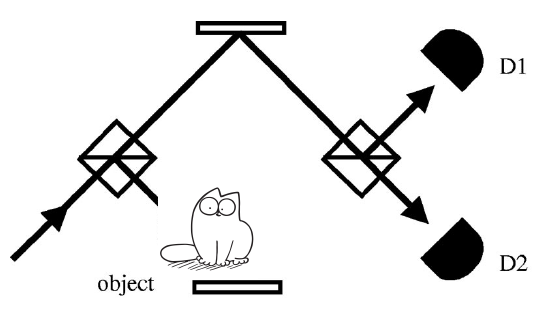
\includegraphics[scale=0.35]{images/ifm2.png}
\caption{The interferometer with an object in one arm.}
\end{figure}

Determine the efficiency of the interaction-free measurement, which is defined
as the ratio of the probability of interaction-free measurement to the
probability of either measurement or absorption as a function of $R_1$. What is
the upper limit of the efficiency?

\item In an improved arrangement, light is reflected through a series of beam
splitters as shown in Fig. 4. If the reflectivity of each beam splitter in the
series is $R=\cos^2(\pi/(2N))$, where $N$ is the number of beam splitters, show
that light will always reach the first detector (D1).

\begin{figure}[h!]
\centering
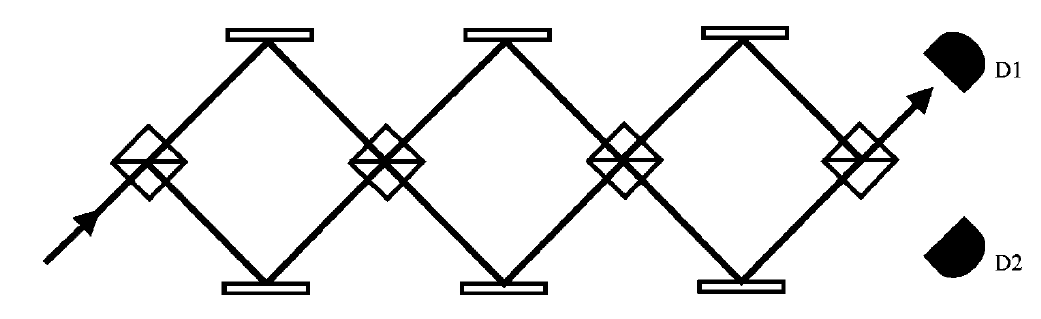
\includegraphics[scale=0.35]{images/ifm3.png}
\caption{The interferometer described in c) for $N=4$.}
\end{figure}

\item If an object blocks all of the upper arms of the interferometer in Fig. 4, a photon
can also be absorbed or reach the second detector. Determine the efficiency of
interaction-free measurement as a function of the number of beam splitters.
\end{enumerate}

\end{document}
